\section{Overview}
\begin{figure}
  \centering
  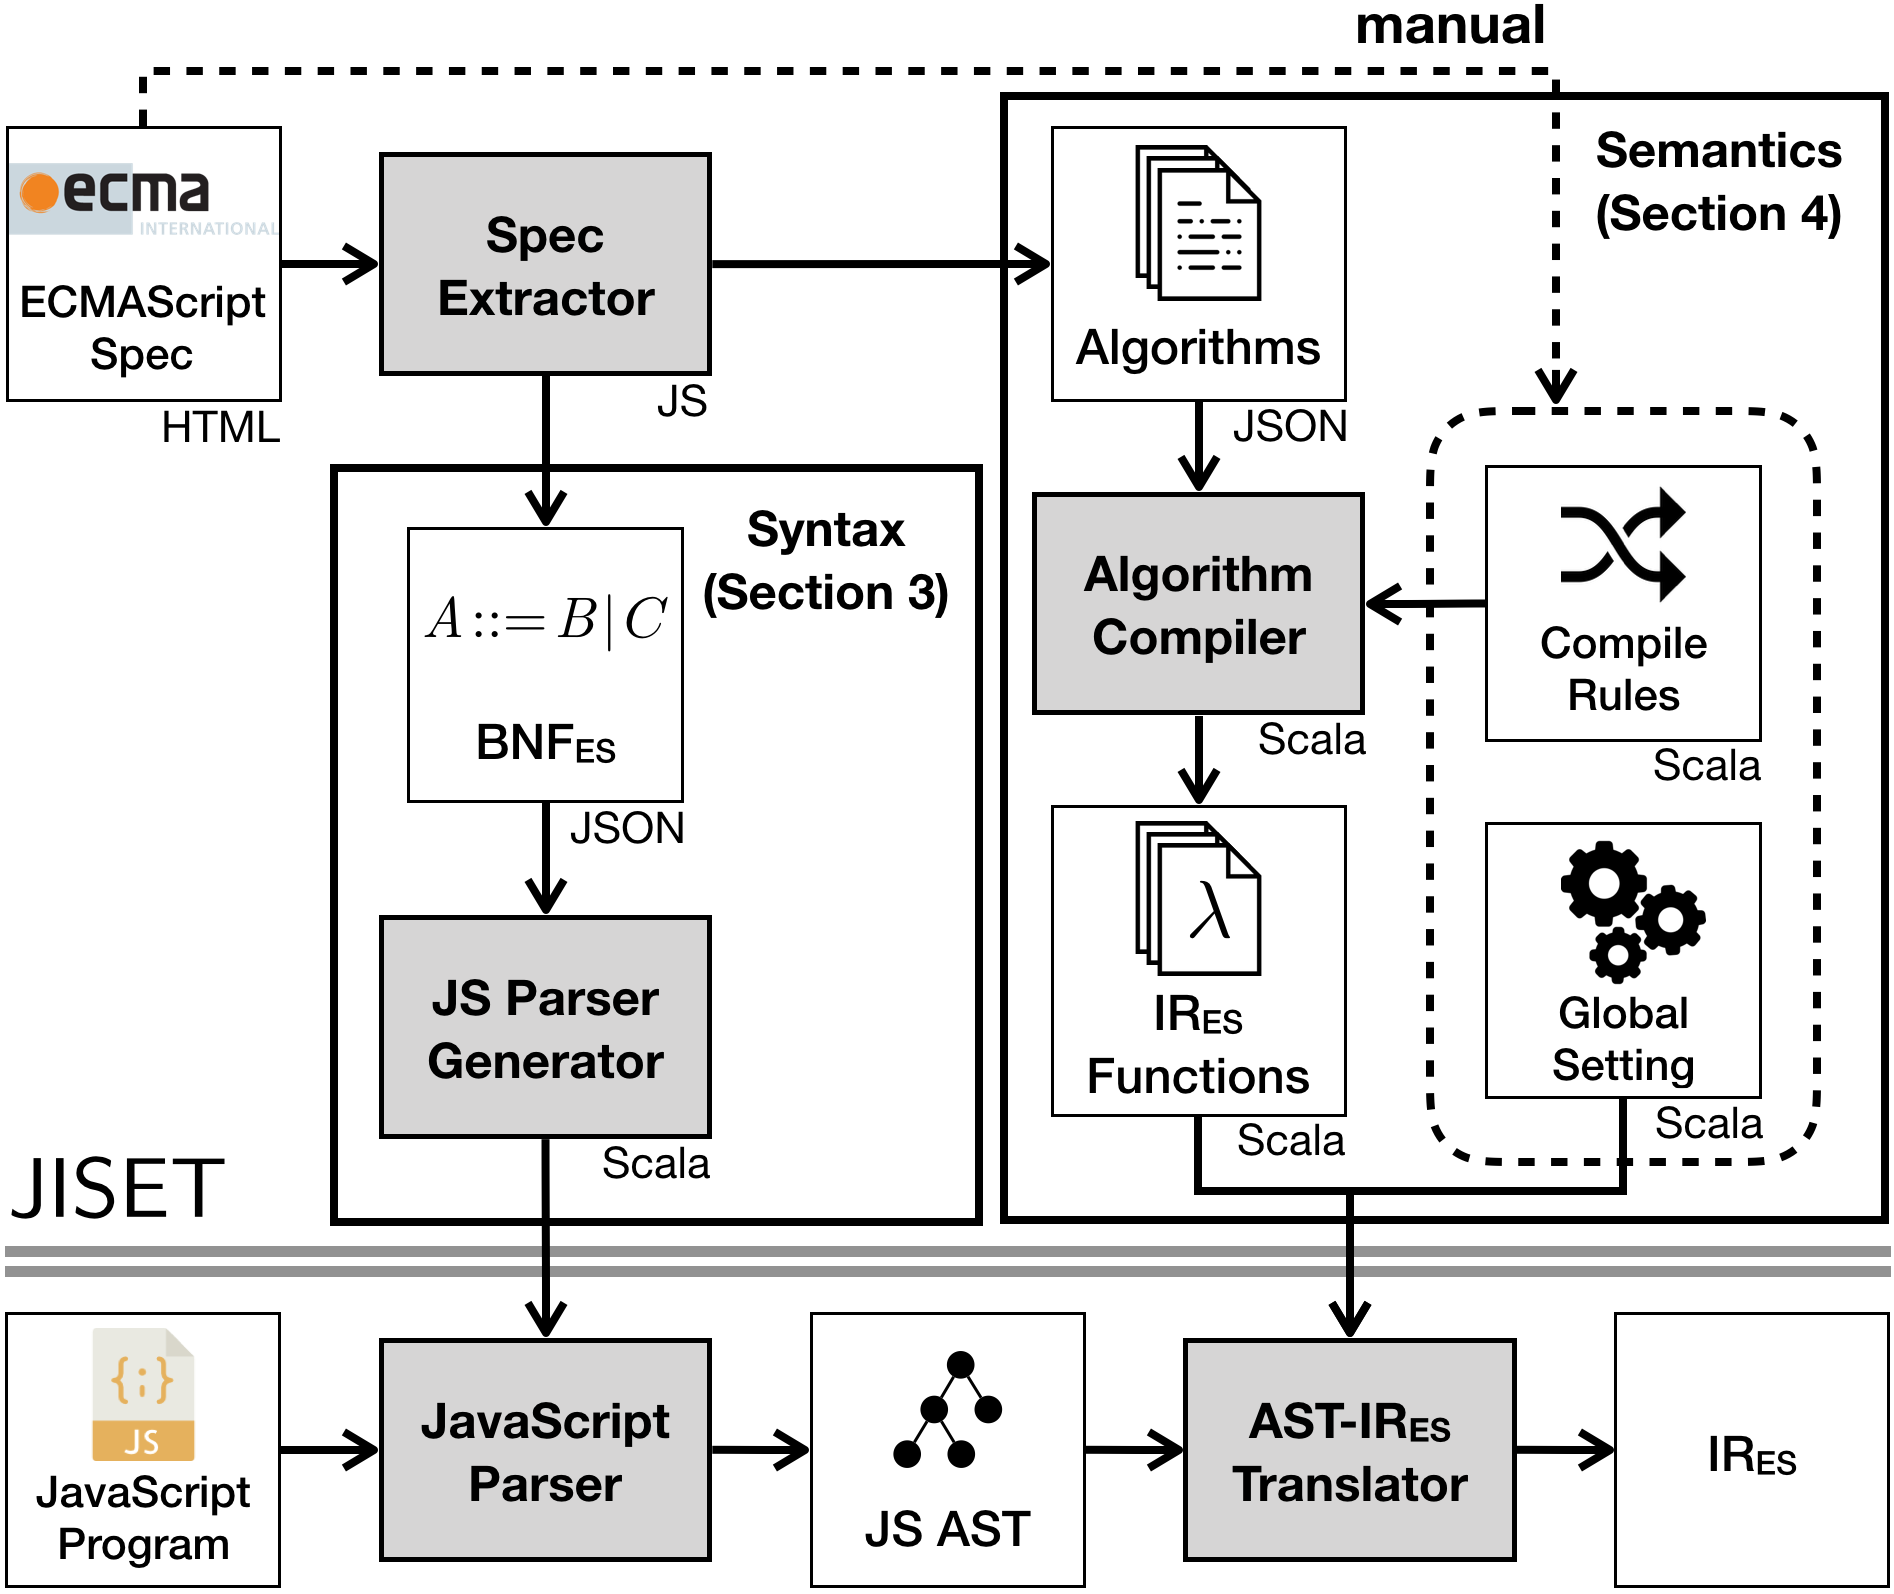
\includegraphics[width=0.48\textwidth]{img/overview.png}
  \caption{Overall structure of \( \tool \): Automatic extraction of
IR-based semantics for ECMAScript}
  \label{fig:overview}
\vspace*{-1em}
\end{figure}

In this section, we introduce the overall structure of \( \tool \)
depicted in Figure~\ref{fig:overview} and the outline of the paper.
Compared to the existing approaches shown in
Figure~\ref{fig:existing}, \( \tool \) automatically generates
{\sf JavaScript Parser} and {\sf AST-\( \ires \) Translator} from the
ECMAScript specification.  Inside \( \tool \), {\sf Spec Extractor}
extracts the JavaScript syntax to build the parser and its semantics
to build the translator.

The motivation of automatically extracting syntax and semantics
of JavaScript from the ECMAScript specification is twofold: 1) the
natural language used in the specification follows well-organized
specific patterns, and 2) the specification is available as HTML files
using various HTML tags.  As the first step, we developed {\sf Spec Extractor}
in JavaScript, which extracts the syntax and semantics from the
ECMAScript specification in HTML into JSON format.

\begin{figure}
  \centering
  \begin{subfigure}[t]{0.4\textwidth}
    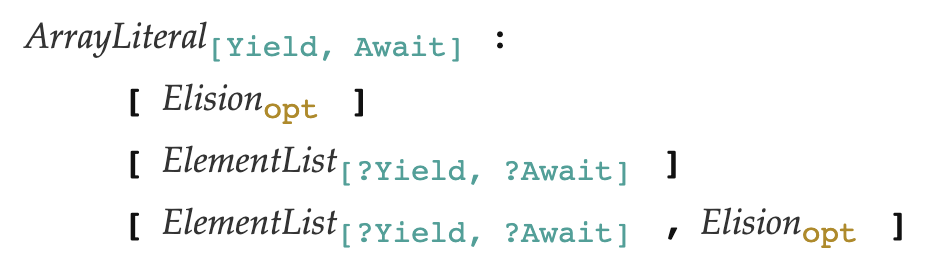
\includegraphics[width=\textwidth]{img/array_literal.png}
    \caption{The \textit{ArrayLiteral} production in ECMAScript 2020}
    \label{fig:array-literal-es}
  \end{subfigure}
  \begin{subfigure}[t]{0.46\textwidth}
    \begin{lstlisting}[style=myScalastyle]
type P[T] = List[Boolean] => LAParser[T]
lazy val ArrayLiteral: P[ArrayLiteral] = memo {
  case List(Yield, Await) =>
  "[" ~ opt(Elision) ~ "]" ^^ ArrayLiteral0 |
  "[" ~ ElementList(Yield, Await) ~ "]" ^^ ArrayLiteral1 |
  "[" ~ ElementList(Yield, Await) ~ "," ~ opt(Elision) ~ "]" ^^ ArrayLiteral2
}
    \end{lstlisting}
    \caption{The generated parser for the \textit{ArrayLiteral} production}
    \label{fig:array-literal-parser}
  \end{subfigure}
  \caption{The \textit{ArrayLiteral} production in the ECMAScript 2020 specification and its generated parser}
  \label{fig:array-literal}
\end{figure}

\smallskip

\textbf{Syntax.} The ECMAScript specification provides the lexical and
syntactic grammars in Appendix A using their own extended Backus-Naur
Form (BNF) for ECMAScript.  We dub it \( \bnfes \) and formally define
it in Section~\ref{sec:parser}.  Our {\sf Spec Extractor} reads the
grammars written in \( \bnfes \) and converts them into JSON files.
For example, Figure~\ref{fig:array-literal}(a) shows the
\textit{ArrayLiteral} production in the ECMAScript 2020
specification.  It takes two boolean parameters \textsf{Yield} and
\textsf{Await} and has three alternatives.  The first alternative
consists of three symbols: two terminal symbols \( \code{[} \) and
\( \code{]} \) and one non-terminal symbol \textit{Elision}$_{\mbox{\footnotesize opt}}$.
The {\small opt} subscript denotes that it is optional.  In the second
and third alternatives, \textit{ElementList}$_{\mbox{\footnotesize\sf [?Yield, ?Await]}}$
denotes a parametric non-terminal symbol \textit{ElementList}
with the parameters \textsf{Yield} and \textsf{Await} of
\textit{ArrayLiteral} as its two arguments. The prefix \textsf{\small ?}
of a symbol denotes that the symbol is passed as an argument.

\begin{figure*}[t]
  \centering
  \begin{subfigure}{0.4\textwidth}
    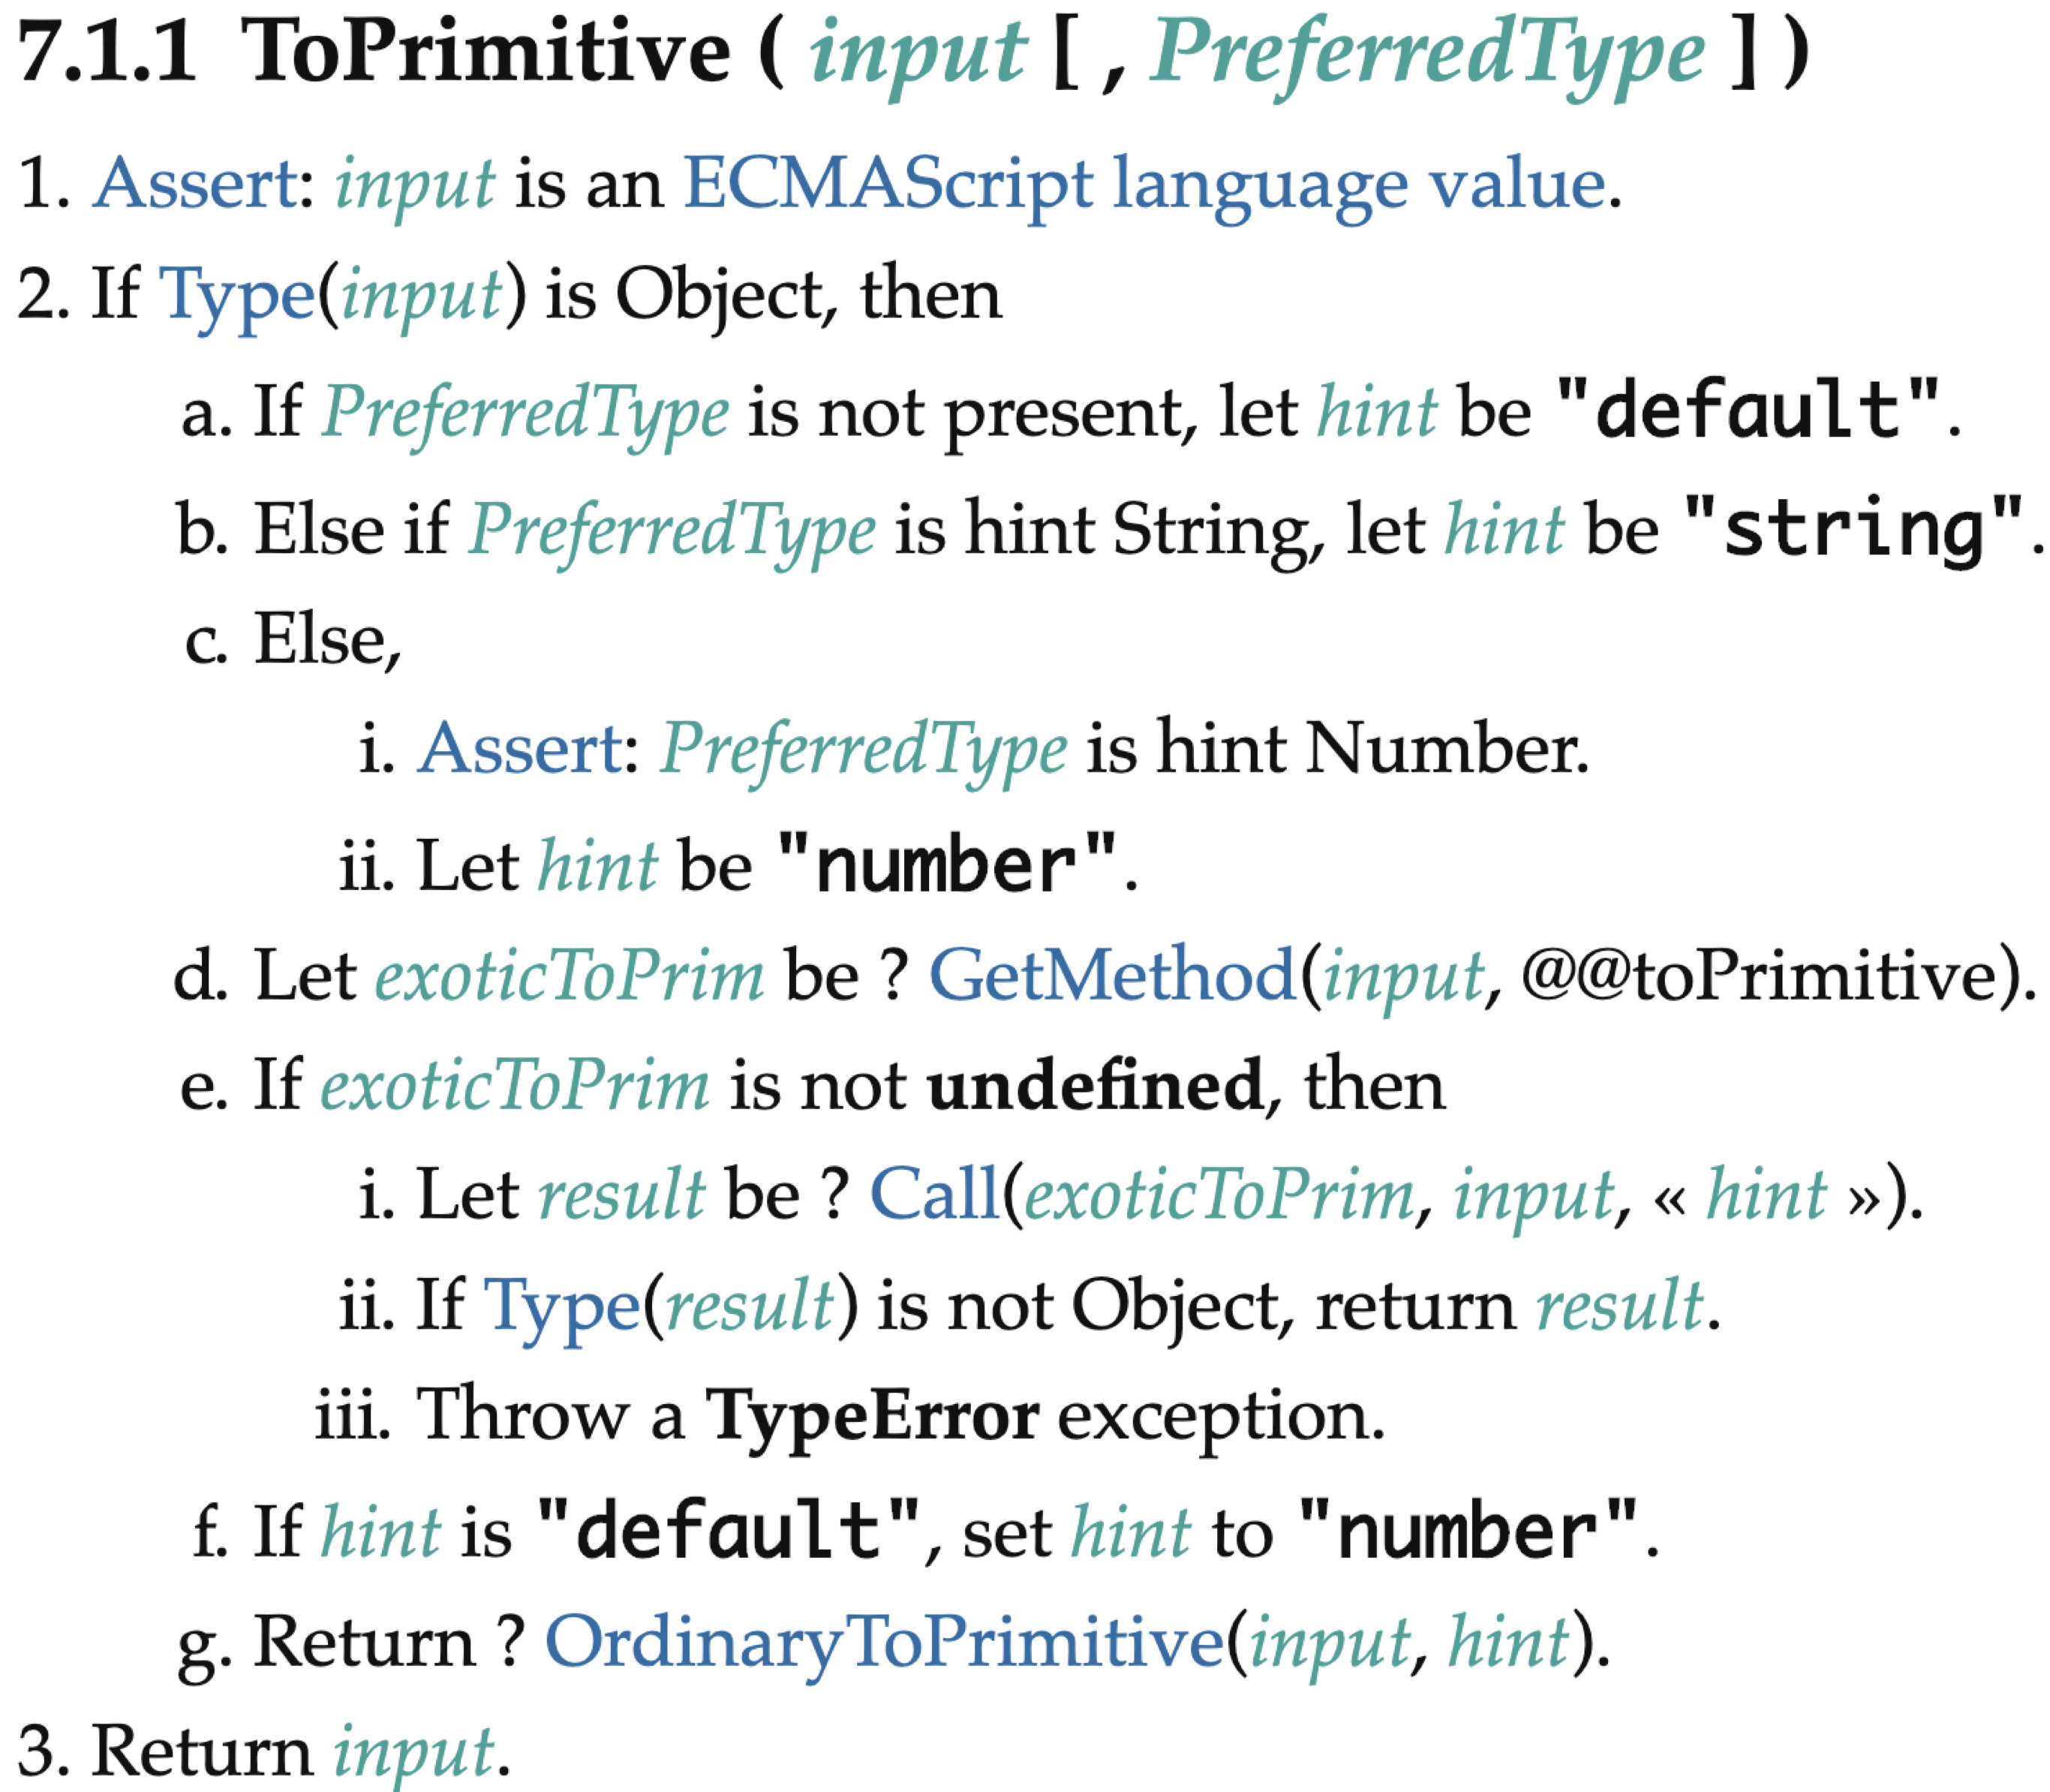
\includegraphics[width=\textwidth]{img/to_primitive.png}
    \subcaption{The \textbf{ToPrimitive} algorithm in ECMAScript 2020}
    \label{fig:to-primitive-es}
  \end{subfigure}
  \qquad
  \begin{subfigure}{0.48\textwidth}
    \begin{lstlisting}[style=ires]
"ToPrimitive" (input, PreferredType) => {
  if (= (Type input) "Object") {
    if (= PreferredType absent) let hint = "default"
    else if (= PreferredType "String") let hint = "string"
    else let hint = "number"
    let exoticToPrim = ? (GetMethod input SYMBOL_toPrimitive)
    if (! (= exoticToPrim undefined)) {
      let result = ? (Call exoticToPrim input (new [hint]))
      if (! (= (Type result) "Object")) return result
      return (Throw INTRINSIC_TypeErrorPrototype)
    }
    if (= hint "default") hint = "number"
    return ? (OrdinaryToPrimitive input hint)
  }
  return input
}
    \end{lstlisting}
    \subcaption{The generated \( \ires \) function for the \textbf{ToPrimitive} algorithm}
    \label{fig:to-primitive-ires}
  \end{subfigure}
  \caption{The \textbf{ToPrimitive} abstract algorithm in the ECMAScript 2020 specification and its generated \( \ires \) function}
  \label{fig:to-primitive}
\end{figure*}

To generate {\sf JavaScript Parser} from a given \( \bnfes \) grammar, we
construct \textsf{JS Parser Generator} in Scala.  It synthesizes a
JavaScript parser according to the given \( \bnfes \), and the
generated parser is defined with Scala parser combinators~\cite{scala-parser-combinators}.
Moreover, in order to parse \( \bnfes \) grammars correctly and
efficiently, we propose \textit{lookahead parsers}, which keep track
of lookaheads, sets of possible next tokens.  With lookahead parsers,
generated parsers become more readable and have one-to-one
mapping to their corresponding grammar productions.
For example, Figure~\ref{fig:array-literal}(b) shows the generated
parser for the \textit{ArrayLiteral} production in Figure~\ref{fig:array-literal}(a).
Each parser has the \( \code{List[Boolean] => LAParser[T]} \) type
because  each production in \( \bnfes \) is parametric with boolean values.
The \( \code{memo} \) is a memoization function for pairs of boolean
parameters and resulting parsers for performance optimization.
The lazy value \( \code{ArrayLiteral} \) corresponds to the
\textit{ArrayLiteral} production.  In the parser, each string literal
such as \( \code{"["} \) or \( \code{"]"} \) denotes a parser for a
terminal symbol.  The \( \code{opt} \) helper function creates
optional parsers.  The parametric non-terminal \textit{ElementList}
with arguments \textsf{Yield} and \textsf{Await} is represented as a
function call \( \code{ElementList(Yield, Await)} \).
The \( \code{\textasciitilde} \) operator combines two parsers
and the \( \code{\^{}\^{}} \) operator describes how to construct ASTs.
When the left-hand side of \( \code{\^{}\^{}} \) is matched, its
right-hand side shows a corresponding AST constructor, where each
constructor has a number denoting the order among alternatives.
For example, the \( \code{ArrayLiteral0} \) constructor corresponds to
the first alternative of the \textit{ArrayLiteral} production.

\smallskip

\textbf{Semantics.}
The ECMAScript specification describes the language semantics as
abstract algorithms in English.  While they are written in a natural
language, the writing style is well-organized with ordered steps and
tagged tokens.  Our {\sf Spec Extractor} reads each abstract algorithm
with HTML tags and converts them into JSON files.  For example,
Figure~\ref{fig:to-primitive}(a) presents the \textbf{ToPrimitive}
abstract algorithm in ECMAScript 2020.  It has three steps and the
second step consists of seven sub-steps.  In the HTML files describing
the abstract algorithms, each parameter or local variable such as
\textit{input} or \textit{PreferredType} has the \( \code{<var>} \)
HTML tag and each value has the \( \code{<code>} \) tag.

%because we utilize tag information to discriminate different kinds of tokens.
To translate such abstract algorithms into representations that are
suitable for manipulation, we define \( \ires \), a specialized
intermediate representation for ECMAScript abstract algorithms.  Then,
we develop \textsf{Algorithm Compiler} in Scala using Scala parser
combinators again to convert given abstract algorithms to \( \ires \)
functions.  It also takes \textsf{Compile Rules} as another input,
which has two parts: parsing rules and conversion rules from each rule to its
corresponding \( \ires \) component.  They are \textit{manually} specified for
the ECMAScript specification; we explain them in detail in
Section~\ref{sec:compiler}.  Thus, each abstract algorithm is
converted into a function written in \( \ires \) via \textsf{Algorithm Compiler}.
For example, Figure~\ref{fig:to-primitive}(b) presents the generated
\( \ires \) function for the \textbf{ToPrimitive} abstract algorithm.
The \( \code{ToPrimitive} \) function takes two parameters:
\( \code{input} \) and \( \code{PreferredType} \).  The optional
\( \code{PreferredType} \) parameter in the abstract algorithm has
a special value \( \code{absent} \) in the generated \( \ires \) function.
Thus, we convert the condition of the 2-a step,
``If \textit{PreferredType} is not present,'' into the equality check
with \( \code{absent} \): \( \code{if (= PreferredType absent)} \).
In this paper, we omit assertions for presentation brevity; we believe
that they can be handled similarly.  Some specific keywords are
represented as string values.  For instance, ``hint Number'' and
``hint String'' are converted into \( \code{"Number"} \) and
\( \code{"String"} \), respectively.  In addition,
\textsf{Algorithm Compiler} modifies prefixes of symbols from
\( \code{@@} \) to \( \code{SYMBOL\_} \) and handles exceptions with
their corresponding intrinsic error objects.

Finally, \( \tool \) constructs {\sf AST-\( \ires \) Translator} with
the given \( \ires \) functions and \textit{manually} specified
{\sf Global Setting}, which have minor but necessary information to
evaluate JavaScript programs described in the ECMAScript specification.
They consists of the structure of the standard built-in
objects and ECMAScript data types.

Putting them all together, we can translate a given JavaScript program
into \( \ires \) via generated {\sf JavaScript Parser} and
{\sf AST-\( \ires \) Translator} by \( \tool \).
Once \( \tool \) provides the entire infrastructure, supporting yet
another ECMAScript version would not require much manual efforts;
the only additional efforts may be possible changes in \textsf{Compile Rules}
and {\sf Global Setting}.

\smallskip

\textbf{Outline.}
In the remainder of this paper, we describe the detailed techniques of
\( \tool \).  We first formally define \( \bnfes \) and how to
automatically generate parsers from given \( \bnfes \) using lookahead
parsers (Section~\ref{sec:parser}).  Then, we explain how to compile
abstract algorithms with tagged tokens into \( \ires \) functions using
compile rules, and introduce a rule generation assistant to
easily construct compile rules (Section~\ref{sec:compiler}).  After
describing implementation details (Section~\ref{sec:impl}),
we evaluate the effectiveness of \( \tool \)
(Section~\ref{sec:eval}), discuss related work
(Section~\ref{sec:related}), and conclude (Section~\ref{sec:conclude}).
